\documentclass[12pt,a4paper]{article}

\usepackage[utf8]{inputenc}
\usepackage[T5]{fontenc}
\usepackage[vietnamese]{babel}
\usepackage{amsmath, amssymb}
\usepackage{graphicx}
\usepackage{float}
\usepackage{booktabs}
\usepackage{hyperref}
\usepackage{geometry}
\geometry{a4paper, margin=2.5cm}

\begin{document}

%========================================
\begin{titlepage}
    \centering

    {\Large \textbf{ĐẠI HỌC BÁCH KHOA}}\\[0.3cm]
    {\large Khoa Khoa học và Kỹ thuật Máy tính}\\[1.5cm]

    \rule{\textwidth}{0.4pt}\\[1cm]

    {\LARGE \textbf{Bài tập --- Phân loại ảnh với các mô hình học sâu cơ bản}}\\[1cm]

    {\large Học sâu và ứng dụng trong thị giác máy tính}\\[0.3cm]
    {\large Mã môn học: CO5085}\\[1cm]

    \rule{\textwidth}{0.4pt}\\[1.5cm]

    % Thông tin nhóm
    {\large \textbf{Nhóm: 2}}\\[0.5cm]

    \textbf{Thành viên:}\\
    Lý Minh Trung - MSHV: 2570349\\
    Ngô Nhất Toàn - MSHV: 2570515\\
    Nguyễn Thái Thành Đạt - MSHV: 2570387\\[1.5cm]

    % Thông tin học kỳ và giảng viên
    \begin{tabular}{rl}
        \textbf{Năm học \& Học kỳ:} & 2025--2026, Học kỳ 2 \\
        \textbf{Giảng viên:} & ThS. Lê Thành Sách \\
    \end{tabular}

    \vfill
    {\large \today}

\end{titlepage}

%========================================
\pagenumbering{arabic}

%========================================
\tableofcontents
\newpage

%========================================
% !TeX root = ../main.tex
\section{Giới thiệu}

\subsection{Mục tiêu của bài báo cáo}

Trong những năm gần đây, học sâu (deep learning) đã trở thành một trong những hướng tiếp cận quan trọng và hiệu quả nhất trong lĩnh vực thị giác máy tính (computer vision). Nhờ khả năng tự động học đặc trưng từ dữ liệu, các mô hình học sâu đã đạt được những kết quả vượt trội trong nhiều bài toán như phân loại ảnh, phát hiện đối tượng và nhận dạng khuôn mặt. Đặc biệt, sự phát triển của các kiến trúc hiện đại như Convolutional Neural Networks (CNN) \cite{vaswani2017attention} và Vision Transformer (ViT) \cite{dosovitskiy2020image} đã mở ra nhiều hướng nghiên cứu và ứng dụng mới.

Bài báo cáo này tập trung vào bài toán phân loại ảnh, một trong những bài toán cơ bản nhưng mang tính nền tảng trong thị giác máy tính. Mục tiêu chính là xây dựng, huấn luyện và so sánh hiệu năng của nhiều mô hình học sâu khác nhau, từ các mô hình đơn giản như \textbf{Softmax Regression} và \textbf{Multi-Layer Perceptron (MLP)} đến các mô hình phức tạp hơn như \textbf{CNN} và \textbf{Vision Transformer}. Thông qua đó, người thực hiện có thể hiểu rõ hơn về cách các mô hình học được biểu diễn dữ liệu ảnh cũng như ưu, nhược điểm của từng kiến trúc.

Bên cạnh việc sử dụng các thành phần có sẵn trong thư viện PyTorch \cite{paszke2019pytorch}, báo cáo còn đi sâu vào việc tự hiện thực một số thành phần quan trọng, điển hình là khối Transformer Encoder. Điều này giúp làm rõ cơ chế hoạt động bên trong của mô hình Transformer, từ đó nâng cao khả năng hiểu và tùy biến mô hình cho các bài toán thực tế.

Ngoài ra, báo cáo cũng khảo sát các hướng mở rộng như kết hợp nhiều kiến trúc khác nhau (ví dụ CNN kết hợp Transformer), các phương pháp biểu diễn ảnh đa dạng, cũng như áp dụng các mô hình chuỗi như LSTM \cite{vennerod2021lstm}, GRU \cite{chung2014empirical} cho dữ liệu ảnh. Những thử nghiệm này nhằm mục đích khám phá sâu hơn không gian thiết kế mô hình và đánh giá ảnh hưởng của từng lựa chọn đến hiệu năng tổng thể.

Thông qua quá trình thực nghiệm và phân tích, báo cáo hướng đến việc cung cấp một cái nhìn toàn diện về các phương pháp tiếp cận khác nhau trong bài toán phân loại ảnh, đồng thời rút ra những nhận xét và bài học quan trọng trong việc xây dựng và đánh giá mô hình học sâu.

\subsection{Giới thiệu về tập dữ liệu CIFAR-10}

Trong bài báo cáo này, nhóm sử dụng tập dữ liệu \textbf{CIFAR-10} \cite{krizhevsky2009learning} để thực hiện các thí nghiệm phân loại ảnh. CIFAR-10 là một trong những tập dữ liệu phổ biến và tiêu chuẩn trong lĩnh vực thị giác máy tính, thường được sử dụng để đánh giá hiệu năng của các mô hình học máy và học sâu.

\subsubsection{Lý do lựa chọn CIFAR-10}

Việc lựa chọn CIFAR-10 cho bài toán này dựa trên một số lý do chính sau:

\begin{itemize}
\item \textbf{Phù hợp với mục tiêu bài tập:} CIFAR-10 có độ phức tạp vừa phải, đủ để thể hiện sự khác biệt giữa các mô hình như MLP, CNN và Transformer, nhưng vẫn có thể huấn luyện trong thời gian hợp lý.
\item \textbf{Dữ liệu chuẩn và phổ biến:} Đây là benchmark phổ biến, giúp dễ dàng so sánh kết quả với các nghiên cứu và triển khai trước đó.
\item \textbf{Kích thước nhỏ gọn:} Ảnh có kích thước nhỏ giúp giảm chi phí tính toán, phù hợp với môi trường thực nghiệm hạn chế tài nguyên.
\item \textbf{Đa dạng về đặc trưng hình ảnh:} Bao gồm nhiều loại đối tượng với đặc trưng khác nhau (động vật, phương tiện), giúp đánh giá khả năng trích xuất đặc trưng của mô hình.
\end{itemize}

Ngoài ra, theo quan sát từ quá trình thực nghiệm của nhóm, CIFAR-10 cũng cho thấy sự khác biệt rõ ràng về hiệu năng giữa các kiến trúc mô hình, từ đó giúp việc phân tích và so sánh trở nên trực quan và có ý nghĩa hơn.

\subsubsection{Đặc trưng của dữ liệu hình ảnh}

CIFAR-10 là tập dữ liệu gồm tổng cộng \textbf{60,000 ảnh màu}, mỗi ảnh có kích thước nhỏ $32 \times 32$ pixel. Tập dữ liệu được chia thành \textbf{10 lớp đối tượng}, bao gồm: airplane, automobile, bird, cat, deer, dog, frog, horse, ship, truck.

Về cách phân chia dữ liệu:
\begin{itemize}
\item \textbf{50,000 ảnh} được sử dụng cho tập huấn luyện (training set)
\item \textbf{10,000 ảnh} còn lại được dùng cho tập kiểm tra (test set)
\end{itemize}

Đặc điểm nổi bật của CIFAR-10 là kích thước ảnh nhỏ nhưng chứa nhiều biến thể về góc nhìn, ánh sáng và nền, khiến bài toán phân loại trở nên không hề đơn giản. Điều này giúp tập dữ liệu trở thành một lựa chọn phù hợp để đánh giá khả năng học đặc trưng của các mô hình từ cơ bản đến nâng cao.

\subsubsection{Phân phối dữ liệu}

Phân phối số lượng mẫu theo từng lớp trong tập huấn luyện CIFAR-10 được minh họa trong Hình~\ref{fig:cifar10_distribution}. 

\begin{figure}[H]
\centering
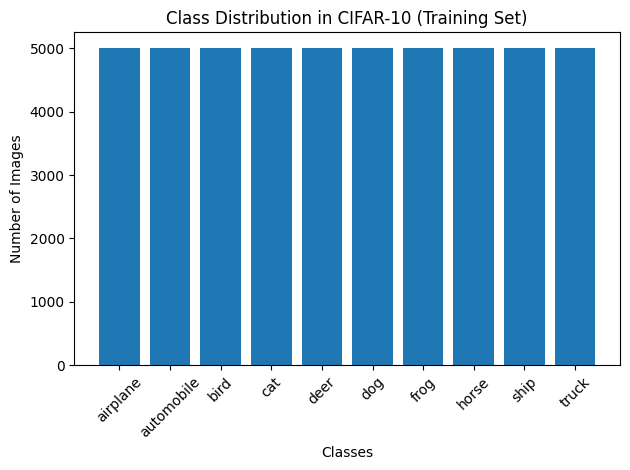
\includegraphics[width=0.7\linewidth]{images/class_distribution_cifar10.png}
\caption{Class distribution of the CIFAR-10 training dataset}
\label{fig:cifar10_distribution}
\end{figure}

Như có thể quan sát, tập dữ liệu CIFAR-10 có phân phối hoàn toàn cân bằng, với mỗi lớp chứa khoảng 5,000 ảnh trong tập huấn luyện. Điều này đảm bảo rằng không có lớp nào chiếm ưu thế trong quá trình huấn luyện, từ đó giúp mô hình học được các đặc trưng một cách công bằng giữa các lớp.

Tính cân bằng của dữ liệu giúp giảm thiểu nguy cơ bias trong mô hình và cho phép việc đánh giá hiệu năng trở nên khách quan hơn. Do đó, trong bài toán này, không cần áp dụng các kỹ thuật xử lý mất cân bằng dữ liệu như oversampling hoặc class weighting.

\subsubsection{Trực quan hóa dữ liệu}

Để hiểu rõ hơn về đặc điểm của tập dữ liệu, một số ảnh mẫu từ mỗi lớp trong CIFAR-10 được trực quan hóa như trong Hình~\ref{fig:cifar10_samples}.

\begin{figure}[H]
\centering
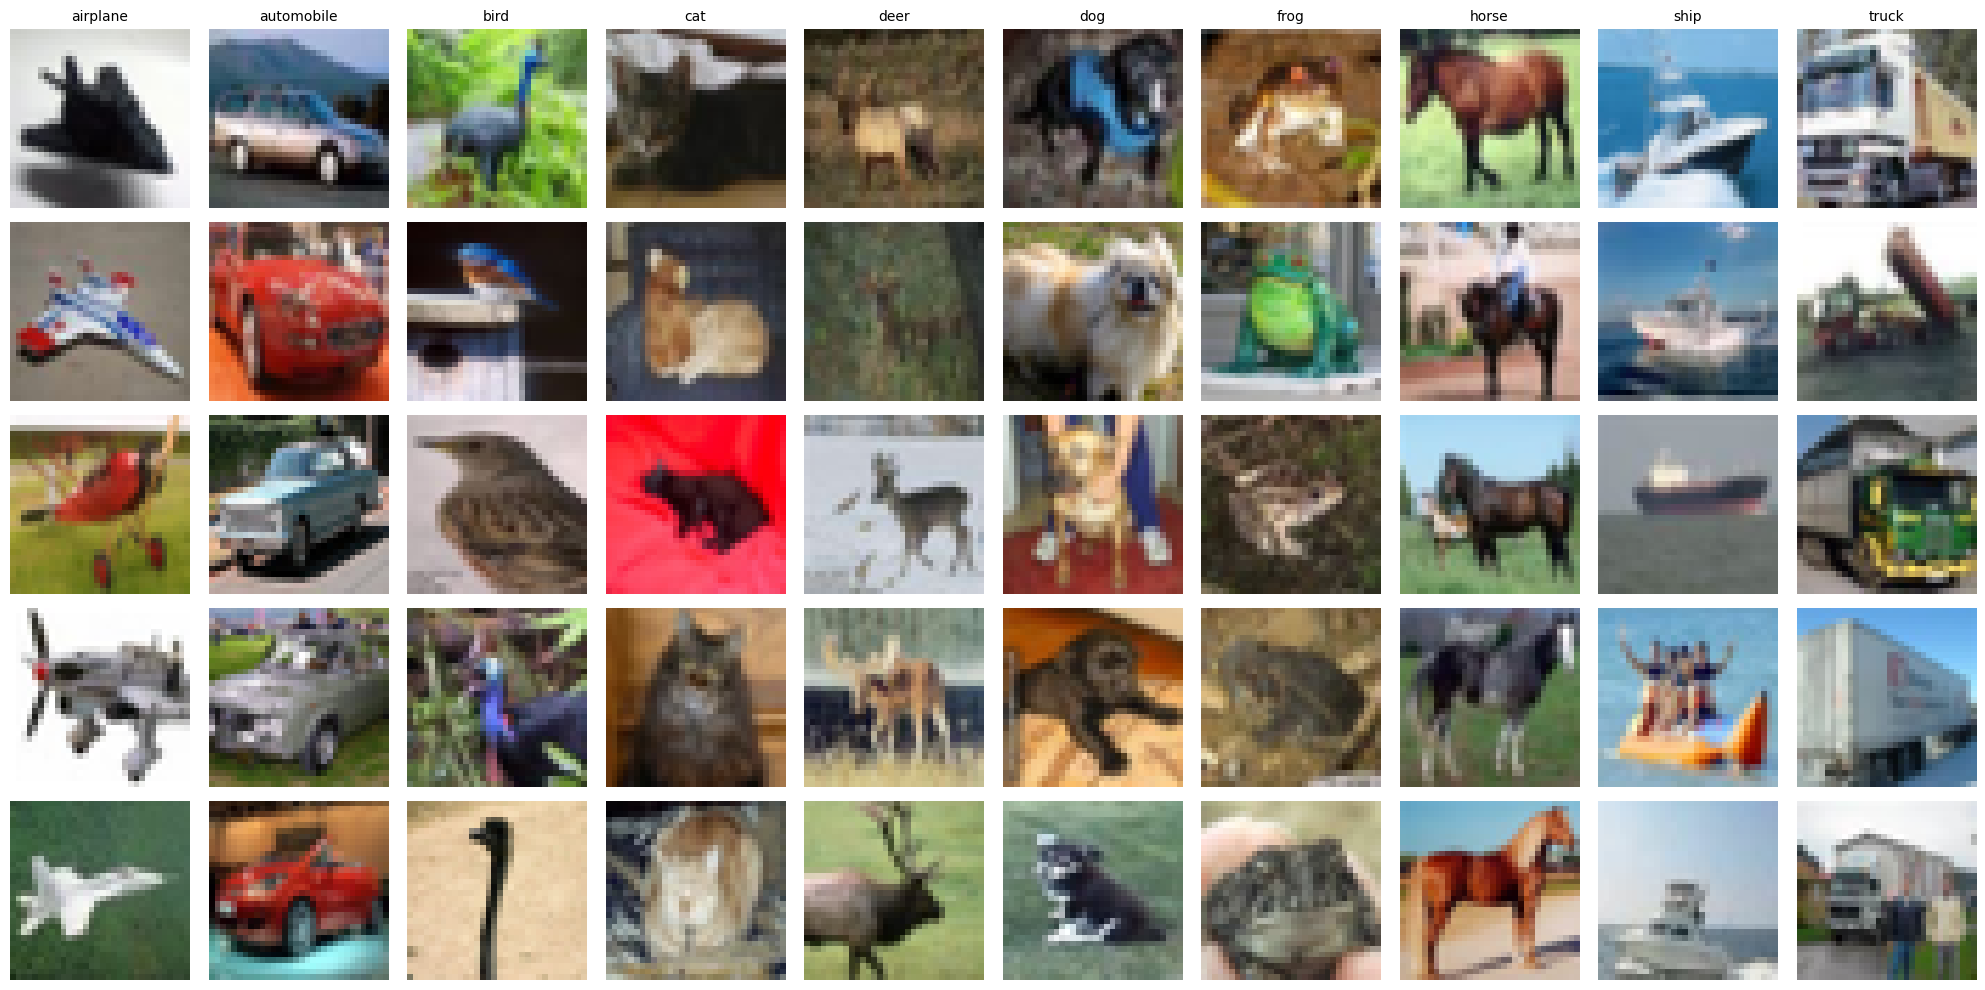
\includegraphics[width=0.9\linewidth]{images/cifar10_samples.png}
\caption{Sample images from each class in CIFAR-10}
\label{fig:cifar10_samples}
\end{figure}

Từ hình trên, có thể nhận thấy rằng các đối tượng trong CIFAR-10 xuất hiện với nhiều biến thể khác nhau về góc nhìn, vị trí và nền. Ngoài ra, các ảnh có độ phân giải thấp (32×32), khiến cho các đặc trưng chi tiết bị hạn chế.

Bên cạnh đó, một số lớp có sự tương đồng về mặt hình ảnh, ví dụ như \textit{cat} và \textit{dog} làm tăng độ khó của bài toán phân loại.

\begin{figure}[H]
\centering
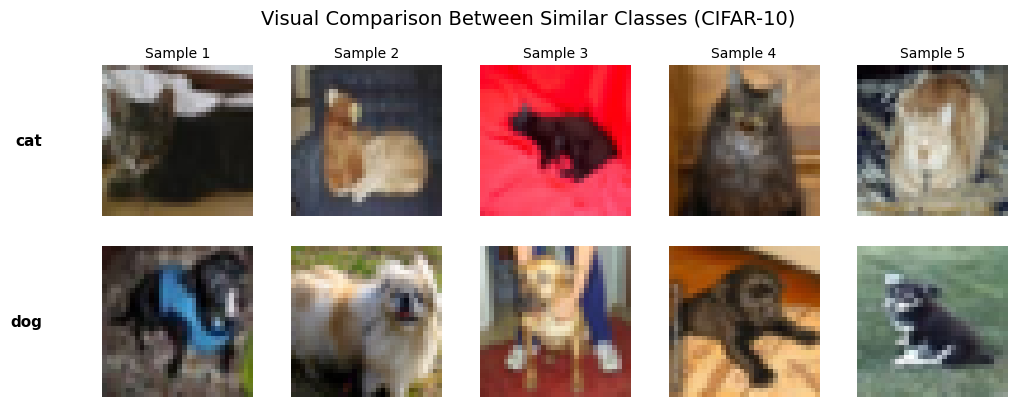
\includegraphics[width=0.9\linewidth]{images/cat_and_dog_visualization.png}
\caption{Sample images from each class in CIFAR-10}
\label{fig:cat_and_dog_visualization}
\end{figure}

Ngoài ra, các ảnh trong CIFAR-10 thường chứa nền đa dạng và phức tạp, trong đó đối tượng chính không phải lúc nào cũng nổi bật hoặc nằm ở vị trí trung tâm. Sự thay đổi về background giữa các ảnh trong cùng một lớp có thể gây nhiễu và làm tăng độ khó trong việc trích xuất đặc trưng.

\begin{figure}[H]
\centering
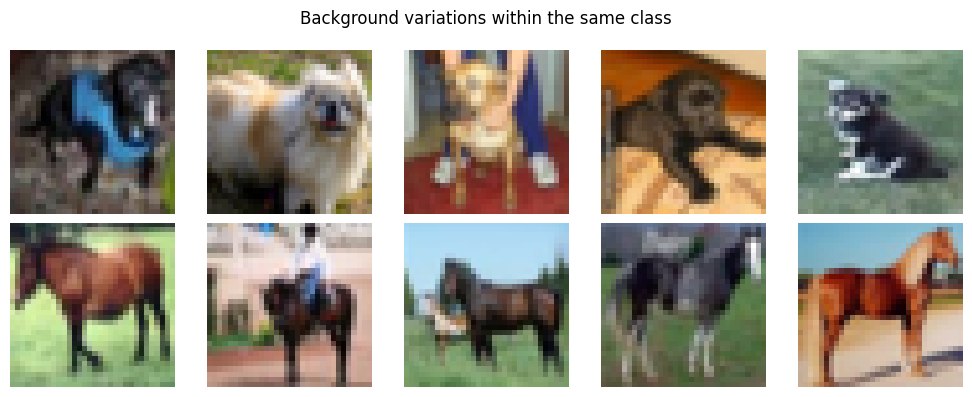
\includegraphics[width=0.9\linewidth]{images/background_variantions.png}
\caption{Examples of background variations within the same class}
\label{fig:background_variations}
\end{figure}

Những đặc điểm này cho thấy rằng mô hình cần có khả năng trích xuất đặc trưng không gian một cách hiệu quả, đồng thời phải đủ mạnh để xử lý sự biến thiên lớn về hình dạng, vị trí và điều kiện nền của đối tượng. 

Cụ thể, mô hình cần học được các biểu diễn mang tính bất biến (invariant) đối với các thay đổi về góc nhìn, tỉ lệ và ánh sáng, đồng thời vẫn phân biệt được các lớp có đặc điểm hình ảnh tương đồng. 

Do đó, các kiến trúc có khả năng khai thác cấu trúc không gian của ảnh, chẳng hạn như các mô hình học sâu dựa trên tích chập hoặc attention, được kỳ vọng sẽ đạt hiệu năng tốt hơn trên tập dữ liệu này.
\section{Xây dụng các mô hình phân loại}

Trong phần này, chúng tôi xây dựng và triển khai bốn mô hình phân loại ảnh bao gồm: Softmax Regression, MLP, CNN và Vision Transformer (ViT). Các mô hình được thiết kế với độ phức tạp tăng dần nhằm đánh giá khả năng học đặc trưng trên tập dữ liệu CIFAR-10.

\subsubsection{Giới thiệu}

Softmax Regression (hay Multinomial Logistic Regression) là một mô hình phân loại tuyến tính được sử dụng cho các bài toán phân loại đa lớp. Mô hình này dự đoán xác suất một mẫu đầu vào thuộc về từng lớp thông qua một phép biến đổi tuyến tính, sau đó lựa chọn lớp có xác suất cao nhất làm kết quả dự đoán.

Do có cấu trúc đơn giản và dễ huấn luyện, Softmax Regression thường được sử dụng làm baseline để so sánh với các mô hình phức tạp hơn.

\subsubsection{Xây dựng kiến trúc}

Dựa trên kiến trúc đã cài đặt, chúng tôi xây dựng mô hình Softmax Regression bằng cách sử dụng một lớp tuyến tính duy nhất để thực hiện phân loại.

Cụ thể, mỗi ảnh đầu vào kích thước $32 \times 32 \times 3$ được làm phẳng thành vector một chiều $x \in \mathbb{R}^{3072}$ thông qua phép reshape trong hàm \texttt{forward}. Vector này sau đó được đưa trực tiếp vào một lớp fully-connected để ánh xạ từ không gian đặc trưng sang không gian nhãn gồm 10 lớp.

Mô hình không sử dụng các lớp ẩn hay hàm kích hoạt phi tuyến, do đó toàn bộ quá trình học chỉ dựa trên một phép biến đổi tuyến tính. Trong quá trình huấn luyện, hàm Softmax được tích hợp trong hàm mất mát (cross-entropy loss) để tính xác suất và tối ưu mô hình.

\begin{itemize}
\item Input: ảnh $32 \times 32 \times 3$
\item Flatten: $x \in \mathbb{R}^{3072}$
\item Linear layer: $3072 \rightarrow 10$
\item Softmax (thông qua hàm loss)
\end{itemize}

\subsubsection{Nhận xét}

Mô hình Softmax Regression có ưu điểm là đơn giản, dễ cài đặt và chi phí tính toán thấp, phù hợp làm baseline cho bài toán phân loại CIFAR-10.

Tuy nhiên, do chỉ sử dụng một phép biến đổi tuyến tính và làm phẳng ảnh đầu vào, mô hình không thể khai thác cấu trúc không gian cũng như các đặc trưng cục bộ của ảnh. Điều này khiến hiệu năng của mô hình bị hạn chế, đặc biệt trong các trường hợp dữ liệu có nhiều biến thể về vị trí, góc nhìn và nền như trong CIFAR-10.

\subsection{Multi-Layer Perceptron (MLP)}

\subsubsection{Giới thiệu}

Multi-Layer Perceptron (MLP) là một kiến trúc mạng neural truyền thẳng (feedforward neural network) bao gồm nhiều lớp fully-connected. Khác với mô hình tuyến tính như Softmax Regression, MLP sử dụng các hàm kích hoạt phi tuyến để học các quan hệ phức tạp hơn trong dữ liệu.

Nhờ khả năng mô hình hóa phi tuyến, MLP có thể học được các biểu diễn trừu tượng và thường đạt hiệu năng tốt hơn so với các mô hình tuyến tính trong các bài toán phân loại.

\subsubsection{Xây dựng kiến trúc}

Dựa trên kiến trúc đã cài đặt, chúng tôi xây dựng một mô hình MLP gồm nhiều lớp fully-connected để thực hiện phân loại ảnh trên tập CIFAR-10.

Cụ thể, mỗi ảnh đầu vào kích thước $32 \times 32 \times 3$ được làm phẳng thành vector một chiều $x \in \mathbb{R}^{3072}$ thông qua phép reshape trong hàm \texttt{forward}. Vector này sau đó được đưa qua các lớp ẩn với kích thước giảm dần, kết hợp với hàm kích hoạt ReLU để học các đặc trưng phi tuyến.

Lớp cuối cùng là một lớp tuyến tính ánh xạ đặc trưng sang không gian nhãn gồm 10 lớp. Tương tự như Softmax Regression, hàm Softmax được tích hợp trong hàm mất mát trong quá trình huấn luyện.

\begin{itemize}
\item Input: ảnh $32 \times 32 \times 3$
\item Flatten: $x \in \mathbb{R}^{3072}$
\item Hidden layer 1: $3072 \rightarrow 512$ + ReLU
\item Hidden layer 2: $512 \rightarrow 256$ + ReLU
\item Output layer: $256 \rightarrow 10$
\item Softmax (thông qua hàm loss)
\end{itemize}

\subsubsection{Nhận xét}

So với Softmax Regression, MLP có khả năng học các quan hệ phi tuyến trong dữ liệu, từ đó cải thiện hiệu năng phân loại. Việc sử dụng nhiều lớp ẩn với kích thước giảm dần giúp mô hình học được các biểu diễn đặc trưng ở nhiều mức độ khác nhau.

Tuy nhiên, tương tự như mô hình tuyến tính, MLP vẫn sử dụng đầu vào dạng vector đã được làm phẳng, dẫn đến việc mất thông tin về cấu trúc không gian của ảnh. Điều này khiến mô hình gặp hạn chế trong việc khai thác các đặc trưng cục bộ quan trọng.

Ngoài ra, số lượng tham số của các lớp fully-connected tương đối lớn, làm tăng nguy cơ overfitting và chi phí tính toán. Do đó, mặc dù MLP mạnh hơn Softmax Regression, nó vẫn chưa phải là lựa chọn tối ưu cho bài toán xử lý ảnh so với các kiến trúc như CNN.

\subsection{Convolutional Neural Network (CNN)}

\subsubsection{Giới thiệu}

Convolutional Neural Network (CNN) là một kiến trúc mạng neural được thiết kế chuyên biệt cho dữ liệu hình ảnh. Khác với các mô hình như MLP, CNN giữ nguyên cấu trúc không gian của ảnh và sử dụng các phép tích chập để học các đặc trưng cục bộ như cạnh, góc và texture.

Nhờ khả năng học đặc trưng phân cấp và tận dụng mối quan hệ không gian giữa các pixel, CNN thường đạt hiệu năng cao trong các bài toán phân loại ảnh.

\subsubsection{Xây dựng kiến trúc}

Đối với bài toán phân loại trên tập CIFAR-10, chúng tôi xây dựng một kiến trúc CNN gồm ba khối tích chập (convolutional blocks) để trích xuất đặc trưng từ ảnh đầu vào kích thước $32 \times 32 \times 3$.

Mỗi khối bao gồm các lớp convolution với kernel kích thước $3 \times 3$, kết hợp với Batch Normalization và hàm kích hoạt ReLU nhằm tăng khả năng học và ổn định quá trình huấn luyện. Sau mỗi khối, lớp MaxPooling được sử dụng để giảm kích thước không gian của feature map.

Cụ thể, kiến trúc được thiết kế như sau:

\begin{itemize}
\item Input: ảnh $32 \times 32 \times 3$

\item \textbf{Block 1:}
\begin{itemize}
\item Conv ($3 \rightarrow 64$), kernel $3 \times 3$
\item Conv ($64 \rightarrow 64$), kernel $3 \times 3$
\item MaxPooling ($32 \rightarrow 16$)
\end{itemize}

\item \textbf{Block 2:}
\begin{itemize}
\item Conv ($64 \rightarrow 128$)
\item Conv ($128 \rightarrow 128$)
\item MaxPooling ($16 \rightarrow 8$)
\end{itemize}

\item \textbf{Block 3:}
\begin{itemize}
\item Conv ($128 \rightarrow 256$)
\item MaxPooling ($8 \rightarrow 4$)
\end{itemize}

\item Flatten: $256 \times 4 \times 4$

\item Fully-connected layers:
\begin{itemize}
\item Linear: $4096 \rightarrow 512$
\item ReLU
\item Linear: $512 \rightarrow 10$
\end{itemize}

\item Dropout ($p = 0.5$) được sử dụng để giảm overfitting
\item Softmax được áp dụng ở đầu ra để thu được xác suất phân lớp
\end{itemize}

\subsubsection{Nhận xét}

Kiến trúc CNN này cho phép mô hình học các đặc trưng hình ảnh theo cấp bậc, từ các đặc trưng đơn giản như cạnh ở các lớp đầu, đến các đặc trưng phức tạp hơn ở các lớp sâu hơn. Điều này đặc biệt phù hợp với tập dữ liệu CIFAR-10, nơi các đối tượng có sự biến đổi lớn về góc nhìn, vị trí và nền.

Việc sử dụng Batch Normalization giúp ổn định quá trình huấn luyện và tăng tốc hội tụ, trong khi Dropout được áp dụng ở các lớp fully-connected nhằm giảm nguy cơ overfitting.

Ngoài ra, cơ chế pooling giúp giảm kích thước feature map và tăng tính bất biến đối với dịch chuyển (translation invariance), từ đó cải thiện khả năng tổng quát hóa của mô hình.

Tuy nhiên, mặc dù CNN có khả năng khai thác đặc trưng cục bộ hiệu quả, mô hình vẫn có thể gặp hạn chế trong việc nắm bắt các mối quan hệ toàn cục trong ảnh, đặc biệt khi đối tượng và ngữ cảnh phân bố phức tạp.

\subsection{Vision Transformer (ViT)}

\subsubsection{Giới thiệu}

Vision Transformer (ViT) là một kiến trúc học sâu áp dụng cơ chế self-attention của Transformer cho bài toán xử lý ảnh. Thay vì sử dụng các phép tích chập như trong CNN, ViT chia ảnh thành các vùng nhỏ (patches) và xử lý chúng như các token trong bài toán xử lý ngôn ngữ tự nhiên.

Thông qua cơ chế self-attention, mô hình có khả năng học được mối quan hệ toàn cục giữa các vùng khác nhau của ảnh, thay vì chỉ tập trung vào các đặc trưng cục bộ. Điều này giúp ViT có tiềm năng biểu diễn mạnh hơn, đặc biệt khi có đủ dữ liệu huấn luyện.

\subsubsection{Xây dựng kiến trúc}

Dựa trên kiến trúc đã cài đặt, chúng tôi xây dựng mô hình Vision Transformer cho bài toán phân loại CIFAR-10 với các thành phần chính như sau:

\paragraph{Patch Embedding}

Ảnh đầu vào kích thước $32 \times 32 \times 3$ được chia thành các patch kích thước $4 \times 4$. Thay vì tách patch thủ công, chúng tôi sử dụng một lớp tích chập với kernel size và stride bằng patch size để thực hiện việc này.

Cụ thể, lớp \texttt{Conv2d} ánh xạ từ 3 kênh đầu vào sang không gian đặc trưng có chiều $dim = 128$, đồng thời giảm kích thước không gian. Kết quả thu được tensor có dạng $(B, dim, H, W)$, sau đó được reshape thành chuỗi các vector patch $(B, N, dim)$.

\paragraph{Token hóa và Positional Embedding}

Một vector đặc biệt (CLS token) được thêm vào đầu chuỗi patch nhằm tổng hợp thông tin toàn cục cho bài toán phân loại. Đồng thời, embedding vị trí (positional embedding) được cộng vào để giữ thông tin về thứ tự không gian của các patch.

\begin{itemize}
\item Số patch: $N = (32 / 4)^2 = 64$
\item Kích thước mỗi token: $dim = 128$
\item Chuỗi đầu vào Transformer: $65$ token (64 patch + 1 CLS)
\end{itemize}

\paragraph{Transformer Encoder}

Chuỗi token được đưa qua một Transformer Encoder gồm $6$ lớp, mỗi lớp bao gồm:
\begin{itemize}
\item Multi-head self-attention với $8$ heads
\item Feed-forward network với kích thước ẩn $256$
\item Dropout để giảm overfitting
\end{itemize}

Cơ chế self-attention cho phép mỗi patch tương tác với tất cả các patch khác, giúp mô hình học được quan hệ toàn cục trong ảnh.

\paragraph{Phân loại}

Sau khi qua Transformer, vector tương ứng với CLS token được trích xuất và đưa qua một lớp chuẩn hóa (LayerNorm) và một lớp tuyến tính để dự đoán nhãn.

\begin{itemize}
\item Input: ảnh $32 \times 32 \times 3$
\item Patch embedding: $4 \times 4$ patches $\rightarrow N = 64$
\item Token dimension: $128$
\item Transformer: $6$ layers, $8$ heads
\item Output: sử dụng CLS token $\rightarrow 10$ lớp
\end{itemize}

\subsubsection{Nhận xét}

Vision Transformer có khả năng mô hình hóa quan hệ toàn cục giữa các vùng trong ảnh thông qua cơ chế self-attention, điều mà các mô hình như MLP hay CNN khó thực hiện trực tiếp.

Tuy nhiên, ViT không có inductive bias mạnh về cấu trúc không gian như CNN (ví dụ: locality hay translation invariance), do đó thường yêu cầu lượng dữ liệu lớn để huấn luyện hiệu quả. Với các tập dữ liệu nhỏ như CIFAR-10, mô hình có thể gặp khó khăn trong việc tổng quát hóa nếu không được regularization hoặc tinh chỉnh phù hợp.

Ngoài ra, chi phí tính toán của self-attention tăng theo bình phương số lượng patch, dẫn đến độ phức tạp cao hơn so với CNN trong nhiều trường hợp.

Tóm lại, ViT là một hướng tiếp cận mạnh mẽ cho bài toán thị giác, nhưng hiệu quả của nó phụ thuộc đáng kể vào quy mô dữ liệu và cách thiết kế mô hình.
\section{Huấn luyện, đánh giá và so sánh}
\section{Tự hiện thực TransformerEncoder và ViT}
% !TeX root = ../main.tex
\section{Các kiến trúc kết hợp và cách embed ảnh khác
nhau}
\section{Mô hình phân loại dựa trên LSTM/GRU}
\section{Tài liệu tham khảo}

\begin{thebibliography}{9}
\bibitem{pytorch} PyTorch Documentation
\end{thebibliography}

%========================================

\end{document}